\documentclass{beamer}  % Creates handouts without notes or animations

% Optional: control how many slides per page (using pgfpages)
%\usepackage{pgfpages}
%\pgfpagesuselayout{2 on 1}[letterpaper,portrait,border shrink=5mm]  % Can be 2 on 1, 4 on 1, or 8 on 1

\usetheme{Madrid}
\usecolortheme{whale}
\setbeameroption{show notes on second screen=right}
\usepackage{graphicx}
\usepackage{fontawesome5}
\usepackage{tikz}
\usetikzlibrary{shapes,arrows}

\title{Policy Conflicts and Strategies in the Policy-Making Process}
\subtitle{Introduction to Public Policy}
\author{David P. Adams, Ph.D.}
\institute{POSC 315 – Week 13}
\date{\today}

\begin{document}

\begin{frame}
    \titlepage
    \note{
        Welcome to this week's lecture on policy conflicts and strategies. Today, we'll dive into:
        \begin{itemize}
            \item The dynamics of policy conflicts
            \item Sources of conflicts
            \item Strategies to manage and resolve them
        \end{itemize}
        This understanding is crucial for anyone looking to engage in public policy effectively.
    }
\end{frame}


\begin{frame}{Learning Objectives}
    \begin{itemize}[<+->]
        \item Understand the \textbf{sources} of policy conflict
            \only<1>{\faIcon{bolt}}
        \item Explore \textbf{strategies} to manage or resolve policy conflicts
            \only<2>{\faIcon{bullseye}}
        \item Reflect on how conflict can serve as both a \textbf{challenge} and an \textbf{opportunity}
            \only<3>{\faIcon{lightbulb}}
        \item Develop a foundation for applying these concepts to \textbf{real-world policy issues}
            \only<4>{\faIcon{check}}
    \end{itemize}
    \note{
        Walk through each objective:
        \begin{itemize}
            \item Sources: We'll examine stakeholder interests, ideological differences, and resource constraints
            \item Strategies: Focus on negotiation, mediation, collaboration, and litigation
            \item Reflection: Help students see both sides of conflict
            \item Application: Use real-world examples throughout
        \end{itemize}
        
        Key points to emphasize:
        \begin{itemize}
            \item These objectives are interconnected
            \item Understanding theory leads to better practice
            \item Real examples will illustrate each concept
        \end{itemize}
    }
\end{frame}

\begin{frame}{What is Policy Conflict?}
    \begin{block}{Definition}
        A situation where stakeholders have opposing interests, goals, or values.
    \end{block}
    
    \begin{columns}[T]
        \begin{column}{0.5\textwidth}
            \textbf{Key Elements:}
            \begin{itemize}
                \item \textbf{Competing Interests}
                \item \textbf{Value Clashes}
                \item \textbf{Limited Resources}
            \end{itemize}
        \end{column}
        \begin{column}{0.5\textwidth}
            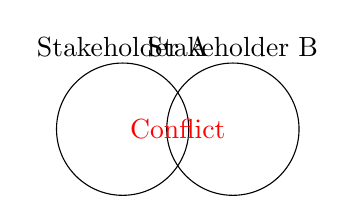
\begin{tikzpicture}[scale=0.7]
                \draw (0,0) circle (1.2);
                \draw (2,0) circle (1.2);
                \node at (0,1.5) {Stakeholder A};
                \node at (2,1.5) {Stakeholder B};
                \node[red] at (1,0) {Conflict};
            \end{tikzpicture}
        \end{column}
    \end{columns}
    \note{
        \begin{itemize}
            \item Policy conflicts emerge when stakeholders—like governments, businesses, or the public—disagree over goals or values.
            \item For instance, balancing economic growth and environmental conservation often results in competing priorities.
        \end{itemize}
    }
\end{frame}

\begin{frame}{Common Sources of Conflict}
    \begin{columns}[T]
        \begin{column}{0.5\textwidth}
            \begin{enumerate}
                \item \textbf{Differing Stakeholder Interests}
                \begin{itemize}
                    \item Business vs. Environmental Goals
                \end{itemize}
                
                \item \textbf{Ideological Differences}
                \begin{itemize}
                    \item Healthcare Debates
                \end{itemize}
            \end{enumerate}
        \end{column}
        \begin{column}{0.5\textwidth}
            \begin{enumerate}\setcounter{enumi}{2}
                \item \textbf{Resource Limitations}
                \begin{itemize}
                    \item Budget Competition
                \end{itemize}
                
                \item \textbf{Regulatory Constraints}
                \begin{itemize}
                    \item Jurisdictional Overlap
                \end{itemize}
            \end{enumerate}
        \end{column}
    \end{columns}
    \note{
        Conflicts can arise for many reasons—stakeholder interests, ideological divides, or practical issues like limited resources or strict regulations. These factors shape the dynamics of policymaking.
    }
\end{frame}

\begin{frame}{Stakeholder Interest Conflicts}
    \begin{block}{Environmental Policy Example}
        \begin{itemize}
            \item Conflict: Economic development vs. conservation
            \item Stakeholders: Industry, environmental groups, communities
        \end{itemize}
    \end{block}

    \begin{block}{Social Policy Example}
        \begin{itemize}
            \item Conflict: Equity vs. efficiency in welfare programs
            \item Stakeholders: Taxpayers, beneficiaries, policymakers
        \end{itemize}
    \end{block}
    \note{
        \begin{itemize}
            \item Stakeholder interests often clash over policy priorities. For example, businesses may prioritize profit, while environmental groups focus on sustainability. These conflicts can lead to debates over resource allocation and policy goals.
            \item Let’s consider two examples. In environmental policy, industries often clash with conservationists. Similarly, social policies bring equity and efficiency into tension, particularly in welfare program designs
        \end{itemize}
    }
\end{frame}

\begin{frame}{Ideological Clashes in Policy}
    \begin{block}{Examples}
        \begin{enumerate}
            \item \textbf{Healthcare Reform}
            \begin{itemize}
                \item Individual responsibility vs. collective welfare
            \end{itemize}
            
            \item \textbf{Tax Policies}
            \begin{itemize}
                \item Redistribution vs. growth-oriented strategies
            \end{itemize}
        \end{enumerate}
    \end{block}
    
    \begin{alertblock}{Impact}
        Polarized debates slow policymaking processes
    \end{alertblock}
    \note{
        \begin{itemize}
            \item Ideological differences often shape policy debates. For instance, healthcare reform pits individual responsibility against collective welfare. Similarly, tax policies can prioritize redistribution or growth-oriented strategies.
            \item These debates can lead to gridlock and hinder policy progress.
        \end{itemize}
    }
\end{frame}

\begin{frame}{Limited Resources as a Conflict Source}
    \begin{block}{Definition}
        Insufficient resources create competition among stakeholders
    \end{block}
    
    \begin{exampleblock}{Examples}
        \begin{enumerate}
            \item \textbf{Infrastructure Funding}
            \begin{itemize}
                \item Project prioritization
            \end{itemize}
            
            \item \textbf{Disaster Relief Allocation}
            \begin{itemize}
                \item Balancing urgency and equity
            \end{itemize}
        \end{enumerate}
    \end{exampleblock}
    \note{
        \begin{itemize}
            \item Resource constraints often lead to conflicts over project funding or disaster relief. Stakeholders must balance competing needs and priorities, which can create tensions and delays.
            \item For example, infrastructure projects require careful prioritization, while disaster relief efforts must balance urgency and equity.
            \item Resource limitations often force tough choices. Policymakers must decide how to allocate limited funds, such as prioritizing infrastructure projects or distributing disaster relief equitably.
        \end{itemize}
    }   
\end{frame}

\begin{frame}{Bureaucratic and Regulatory Barriers}
    \begin{columns}[T]
        \begin{column}{0.6\textwidth}
            \begin{block}{Definition}
                Conflicts from overlapping or restrictive regulations
            \end{block}
            
            \begin{exampleblock}{Example}
                Federal vs. state laws on marijuana legalization
            \end{exampleblock}
        \end{column}
        \begin{column}{0.4\textwidth}
            \begin{alertblock}{Impact}
                \begin{itemize}
                    \item Delayed implementation
                    \item Increased litigation costs
                \end{itemize}
            \end{alertblock}
        \end{column}
    \end{columns}
    \note{
        \begin{itemize}
            \item Regulatory conflicts can arise from overlapping or inconsistent laws. For example, federal and state regulations on marijuana legalization often clash, creating confusion and legal challenges.
            \item These conflicts can delay policy implementation and increase costs, as stakeholders navigate complex legal frameworks.
        \end{itemize}
    }
\end{frame}

\begin{frame}{Managing Policy Conflicts}
    \begin{columns}[T]
        \begin{column}{0.5\textwidth}
            \textbf{Key Strategies:}
            \begin{enumerate}
                \item Negotiation \faIcon{handshake}
                \item Mediation \faIcon{users}
                \item Collaboration \faIcon{users}
                \item Litigation \faIcon{gavel}
            \end{enumerate}
        \end{column}
        \begin{column}{0.5\textwidth}
            \begin{alertblock}{Importance}
                Effective management ensures progress and stakeholder satisfaction
            \end{alertblock}
        \end{column}
    \end{columns}
    \note{
        \begin{itemize}
            \item Policymakers can use various strategies to manage conflicts effectively. Negotiation, mediation, collaboration, and litigation offer different approaches to resolving disputes.
            \item These strategies are essential for maintaining progress and ensuring stakeholder satisfaction.
        \end{itemize}
    }
\end{frame}

\begin{frame}{Negotiation as a Strategy}
    \begin{columns}[T]
        \begin{column}{0.5\textwidth}
            \textbf{Advantages:}
            \begin{itemize}
                \item Cost-effective
                \item Builds relationships
            \end{itemize}
            
            \textbf{Challenges:}
            \begin{itemize}
                \item Power imbalances
                \item Requires trust
            \end{itemize}
        \end{column}
        \begin{column}{0.5\textwidth}
            \begin{exampleblock}{Real-World Example}
                U.S. budget negotiations between Congress and the President
            \end{exampleblock}
        \end{column}
    \end{columns}
    \note{
        \begin{itemize}
            \item Negotiation is a common strategy for resolving policy conflicts. It can be cost-effective and help build relationships among stakeholders.
            \item However, negotiations may face challenges such as power imbalances and the need for trust among parties.
            \item For example, U.S. budget negotiations between Congress and the President require compromise and trust to reach agreements.
            \item Negotiation is often the first step in conflict resolution. It’s cost-effective and fosters relationship-building, but it depends heavily on trust and balanced power dynamics, as seen in budget negotiations between Congress and the President.
        \end{itemize}
    }
\end{frame}

\begin{frame}{Mediation as a Strategy}
    \begin{columns}[T]
        \begin{column}{0.6\textwidth}
            \begin{block}{Definition}
                A neutral third party facilitates discussions to resolve conflicts
            \end{block}
            
            \begin{itemize}
                \item \textbf{Advantages:}
                \begin{itemize}
                    \item Reduces hostility
                    \item Provides structure
                \end{itemize}
                \item \textbf{Challenges:}
                \begin{itemize}
                    \item Depends on mediator skill
                    \item Requires cooperation
                \end{itemize}
            \end{itemize}
        \end{column}
        \begin{column}{0.4\textwidth}
            \begin{exampleblock}{Real Example}
                Labor disputes resolved through federal mediation
                \centering
                \faIcon{balance-scale}
            \end{exampleblock}
        \end{column}
    \end{columns}
    \note{
        \begin{itemize}
            \item Mediation involves a neutral third party facilitating discussions between conflicting parties. It can reduce hostility and provide structure to negotiations.
            \item However, mediation's success depends on the mediator's skill and the willingness of parties to cooperate.
            \item For example, labor disputes are often resolved through federal mediation, which helps parties reach agreements and avoid costly strikes.
        \end{itemize}
    }
\end{frame}

\begin{frame}{Collaboration as a Strategy}
    \begin{columns}[T]
        \begin{column}{0.5\textwidth}
            \begin{block}{Key Elements}
                \begin{itemize}
                    \item Trust and communication
                    \item Shared decision-making
                    \item Resource allocation
                \end{itemize}
            \end{block}
        \end{column}
        \begin{column}{0.5\textwidth}
            \begin{alertblock}{Challenges}
                \begin{itemize}
                    \item High transaction costs
                    \item Power imbalances
                    \item Time-intensive
                \end{itemize}
            \end{alertblock}
        \end{column}
    \end{columns}
    
    \begin{exampleblock}{Real-World Example}
        Skokomish Watershed initiative involving government, nonprofits, and local communities
    \end{exampleblock}
    \note{
        \begin{itemize}
            \item Collaboration requires trust, communication, and shared decision-making among stakeholders. It can help allocate resources effectively and build lasting solutions.
            \item However, collaboration can be challenging due to high transaction costs, power imbalances, and time-intensive processes.
            \item For example, the Skokomish Watershed initiative brought together government, nonprofits, and local communities to develop a sustainable management plan, highlighting the benefits and challenges of collaboration.
            \item Collaboration builds long-term solutions by bringing all stakeholders to the table. It’s resource-intensive but often leads to more durable outcomes, as seen in collaborative watershed management.
        \end{itemize}
    }
\end{frame}

\begin{frame}{Litigation as a Strategy}
    \begin{block}{Definition}
        Resolving policy conflicts through the judicial system
    \end{block}
    
    \begin{columns}[T]
        \begin{column}{0.5\textwidth}
            \textbf{Advantages:}
            \begin{itemize}
                \item Provides definitive resolution
                \item Enforces legal compliance
                \item Sets precedent
            \end{itemize}
        \end{column}
        \begin{column}{0.5\textwidth}
            \textbf{Challenges:}
            \begin{itemize}
                \item Costly and time-consuming
                \item May increase animosity
                \item Limited flexibility
            \end{itemize}
        \end{column}
    \end{columns}
    
    \begin{exampleblock}{Landmark Example}
        \centering
        Brown v. Board of Education (1954)\\
        \faIcon{gavel}
    \end{exampleblock}
    \note{
        \begin{itemize}
            \item Litigation involves resolving policy conflicts through the judicial system. It provides a definitive resolution, enforces legal compliance, and sets precedents for future cases.
            \item However, litigation can be costly, time-consuming, and may increase animosity among stakeholders. It also limits flexibility in finding creative solutions.
            \item For example, the landmark case Brown v. Board of Education (1954) resolved a major policy conflict over school segregation, setting a precedent for desegregation in the U.S.
        \end{itemize}
    }   
\end{frame}

\begin{frame}{Case Study: Skokomish Watershed Initiative}
    \begin{block}{The Conflict}
        Competing interests over natural resource use in the watershed
    \end{block}
    
    \begin{columns}[T]
        \begin{column}{0.5\textwidth}
            \textbf{Resolution Strategy:}
            \begin{itemize}
                \item Multi-stakeholder collaboration
                \item Trust-building exercises
                \item Shared goal setting
            \end{itemize}
        \end{column}
        \begin{column}{0.5\textwidth}
            \textbf{Outcome:}
            \begin{itemize}
                \item Long-term management plan
                \item Balanced interests
                \item Sustainable solution
            \end{itemize}
        \end{column}
    \end{columns}
    \note{
        \begin{itemize}
            \item The Skokomish Watershed initiative addressed conflicts over natural resource use by bringing together multiple stakeholders. Through collaboration, trust-building, and shared goal-setting, the initiative developed a long-term management plan that balanced competing interests and provided a sustainable solution.
            \item The Skokomish Watershed initiative is a successful example of multi-stakeholder collaboration in resolving policy conflicts. By building trust and setting shared goals, the initiative developed a sustainable management plan that balanced competing interests.
            \item This case highlights how collaboration can address complex conflicts involving diverse stakeholders. Trust and communication were central to its success.
        \end{itemize}
    }
\end{frame}

\begin{frame}{Transaction Costs of Collaboration}
    \begin{block}{What are Transaction Costs?}
        Time, resources, and effort invested in collaborative processes
    \end{block}
    
    \begin{columns}[T]
        \begin{column}{0.5\textwidth}
            \textbf{Examples:}
            \begin{itemize}
                \item Long meetings
                \item Trust building
                \item Framework development
            \end{itemize}
        \end{column}
        \begin{column}{0.5\textwidth}
            \begin{alertblock}{Benefits vs. Costs}
                Higher upfront costs but more sustainable long-term outcomes
            \end{alertblock}
        \end{column}
    \end{columns}
    \note{
        \begin{itemize}
            \item Transaction costs refer to the time, resources, and effort invested in collaborative processes. These costs include long meetings, trust-building exercises, and framework development.
            \item While collaboration can be resource-intensive, it often leads to more sustainable long-term outcomes by addressing underlying conflicts and building lasting solutions.
            \item Collaboration is resource-intensive, requiring significant time and effort. However, these upfront investments can lead to lasting solutions and improved stakeholder relationships.
        \end{itemize}
    }
\end{frame}

\begin{frame}{Common Challenges in Conflict Management}
    \begin{columns}[t]
        \begin{column}{0.33\textwidth}
            \centering
            \textbf{Trust Deficit}\\
            \faIcon[3x]{heart-broken}\\
            Lack of faith among stakeholders
        \end{column}
        \begin{column}{0.33\textwidth}
            \centering
            \textbf{Power Imbalances}\\
            \faIcon[3x]{balance-scale}\\
            Dominance of certain groups
        \end{column}
        \begin{column}{0.33\textwidth}
            \centering
            \textbf{Complexity}\\
            \faIcon[3x]{puzzle-piece}\\
            Multi-faceted problems
        \end{column}
    \end{columns}
    \note{
        \begin{itemize}
            \item Conflict management often faces challenges such as a lack of trust among stakeholders, power imbalances, and the complexity of multi-faceted problems.
            \item These challenges can hinder effective resolution and require careful strategies to overcome.
            \item Trust deficits, power imbalances, and complex issues are recurring challenges in conflict management. Overcoming these barriers requires patience and strategic thinking.
        \end{itemize}
    }
\end{frame}

\begin{frame}{Conflict as an Opportunity}
    \begin{columns}[T]
        \begin{column}{0.5\textwidth}
            \begin{itemize}
                \item \textbf{Innovation} \faIcon{lightbulb}
                \begin{itemize}
                    \item Inspires creative solutions
                \end{itemize}
                \item \textbf{Stakeholder Buy-In} \faIcon{users}
                \begin{itemize}
                    \item Builds lasting support
                \end{itemize}
            \end{itemize}
        \end{column}
        \begin{column}{0.5\textwidth}
            \begin{itemize}
                \item \textbf{Strengthened Institutions} \faIcon{building}
                \begin{itemize}
                    \item Enhances capacity
                \end{itemize}
                \item \textbf{Example:} ACA negotiations
            \end{itemize}
        \end{column}
    \end{columns}
    \note{
        \begin{itemize}
            \item Conflict can be an opportunity for innovation, inspiring creative solutions to complex problems. It can also help build stakeholder buy-in, leading to lasting support for policies.
            \item Additionally, conflict can strengthen institutions by enhancing their capacity to address challenges and adapt to changing circumstances.
            \item For example, negotiations over the Affordable Care Act (ACA) led to innovative policy solutions and built support for healthcare reform.
            \item Conflict isn’t always negative. It can drive innovation, strengthen institutions, and create better policy outcomes when managed effectively.
        \end{itemize}
    }
\end{frame}

\begin{frame}{Conflict: A Challenge and Opportunity}
    \begin{columns}[T]
        \begin{column}{0.5\textwidth}
            \begin{alertblock}{Challenges}
                \begin{itemize}
                    \item Distrust
                    \item Inefficiency
                    \item Stalemates
                \end{itemize}
            \end{alertblock}
        \end{column}
        \begin{column}{0.5\textwidth}
            \begin{block}{Opportunities}
                \begin{itemize}
                    \item Better decisions
                    \item Engagement
                    \item Innovation
                \end{itemize}
            \end{block}
        \end{column}
    \end{columns}
    \note{
        \begin{itemize}
            \item Policy conflicts present challenges such as distrust, inefficiency, and stalemates that can hinder progress and lead to negative outcomes.
            \item However, conflicts also offer opportunities for better decisions, increased engagement, and innovation that can lead to positive policy changes and lasting solutions.
            \item By recognizing both the challenges and opportunities of conflict, policymakers can navigate disputes effectively and turn challenges into opportunities for positive change.
            \item Conflict can hinder progress but also serve as a catalyst for meaningful change. Policymakers must learn to harness its potential while minimizing its downsides.
        \end{itemize}
    }
\end{frame}

\begin{frame}{Policy Conflict in Action: ACA}
    \begin{block}{The Conflict}
        Ideological divides over healthcare access and government intervention
    \end{block}
    
    \begin{columns}[T]
        \begin{column}{0.5\textwidth}
            \textbf{Strategies Used:}
            \begin{itemize}
                \item Negotiation
                \item Compromise
                \item Incrementalism
            \end{itemize}
        \end{column}
        \begin{column}{0.5\textwidth}
            \begin{alertblock}{Outcome}
                Landmark legislation with ongoing debates
            \end{alertblock}
        \end{column}
    \end{columns}
    \note{
        \begin{itemize}
            \item The Affordable Care Act (ACA) faced significant policy conflicts due to ideological divides over healthcare access and the role of government intervention.
            \item Policymakers used negotiation, compromise, and incrementalism to address these conflicts and pass landmark healthcare legislation.
            \item The ACA remains a subject of ongoing debates and policy changes, highlighting the complexities of managing policy conflicts in practice.
            \item The ACA is a prime example of how policy conflicts can shape major legislation. Negotiation, compromise, and incrementalism were key strategies in addressing ideological divides and passing the landmark healthcare law.
            \item The ACA’s passage exemplifies the challenges of managing ideological conflict. Incrementalism and compromise were key to its implementation.
        \end{itemize}
    }
\end{frame}

\begin{frame}{Incrementalism as a Conflict Strategy}
    \begin{block}{Definition}
        Small, manageable changes to address public problems
    \end{block}
    
    \begin{columns}[T]
        \begin{column}{0.5\textwidth}
            \textbf{Pros:}
            \begin{itemize}
                \item Stability
                \item Reduced resistance
                \item Easier consensus
            \end{itemize}
        \end{column}
        \begin{column}{0.5\textwidth}
            \textbf{Cons:}
            \begin{itemize}
                \item Slow progress
                \item Limited impact
                \item May delay urgent needs
            \end{itemize}
        \end{column}
        
    \end{columns}
    
    \begin{exampleblock}{Example}
        Climate change policies using gradual carbon reduction targets
    \end{exampleblock}
    \note{
            \begin{itemize}
                \item Incrementalism involves making small, manageable changes to address public problems. It offers stability, reduces resistance, and can lead to easier consensus among stakeholders.
                \item However, incrementalism can result in slow progress, limited impact, and delays in addressing urgent needs. Policymakers must balance these trade-offs when using incremental approaches.
                \item Incrementalism is a common strategy for managing policy conflicts. It involves making small, manageable changes to address public problems, reducing resistance and building consensus over time.
                \item Incrementalism allows policymakers to implement changes gradually, reducing resistance and fostering stability. However, it may fall short when bold action is needed.
            \end{itemize}
        }
\end{frame}


\begin{frame}{Adaptive Management as a Strategy}
    \begin{block}{Definition}
        A flexible, iterative approach to policymaking that allows for adjustments based on feedback and outcomes
    \end{block}
    
    \begin{columns}[T]
        \begin{column}{0.6\textwidth}
            \textbf{Key Principles:}
            \begin{itemize}
                \item Monitor policy outcomes
                \item Incorporate feedback
                \item Maintain flexibility
            \end{itemize}
        \end{column}
        \begin{column}{0.4\textwidth}
            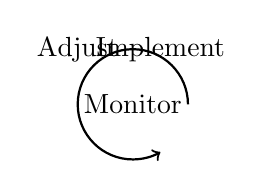
\begin{tikzpicture}[scale=0.7]
                \draw[->,thick] (0,0) arc (0:300:1);
                \node at (-1,0) {Monitor};
                \node at (-2,1) {Adjust};
                \node at (-0.5,1) {Implement};
            \end{tikzpicture}
        \end{column}
    \end{columns}
    
    \begin{exampleblock}{Example}
        Climate change policies adapting to new scientific findings
    \end{exampleblock}
    \note{
        \begin{itemize}
            \item Adaptive management is a flexible, iterative approach to policymaking that allows for adjustments based on feedback and outcomes. It involves monitoring policy outcomes, incorporating feedback, and maintaining flexibility to adapt to changing circumstances.
            \item For example, climate change policies often use adaptive management to respond to new scientific findings and evolving environmental conditions.
            \item Adaptive management is a dynamic approach to policymaking that allows for continuous learning and adjustment. It helps policymakers respond to changing circumstances and improve policy outcomes over time.
            \item Adaptive management focuses on flexibility, allowing policies to evolve in response to real-world challenges. It’s especially useful for complex, dynamic issues like climate change.
        \end{itemize}
    }
\end{frame}

\begin{frame}{Discussing Sources of Policy Conflict}
    \begin{columns}[T]
        \begin{column}{0.5\textwidth}
            \textbf{Sources to Consider:}
            \begin{itemize}
                \item Stakeholder interests \faIcon{users}
                \item Ideological differences \faIcon{brain}
                \item Resource limitations \faIcon{coins}
                \item Regulatory constraints \faIcon{gavel}
            \end{itemize}
        \end{column}
        \begin{column}{0.5\textwidth}
            \begin{block}{Discussion Goal}
                Identify patterns and real-world examples to contextualize conflicts
            \end{block}
        \end{column}
    \end{columns}
    \note{
        \begin{itemize}
            \item Discuss with your peers which source of conflict you find most prevalent and why. Use examples from current events or historical cases to support your argument.
            \item When discussing policy conflicts, consider the various sources that can lead to disagreements among stakeholders. These sources include differing interests, ideological divides, resource constraints, and regulatory challenges.
            \item The goal of this discussion is to identify common patterns and real-world examples that illustrate how these sources of conflict play out in policy debates.
            \item By understanding the sources of policy conflict, you can better analyze and address disputes in your own policy work.
        \end{itemize}
    }
\end{frame}

\begin{frame}{The Conflict Resolution Pyramid}
    \begin{center}
        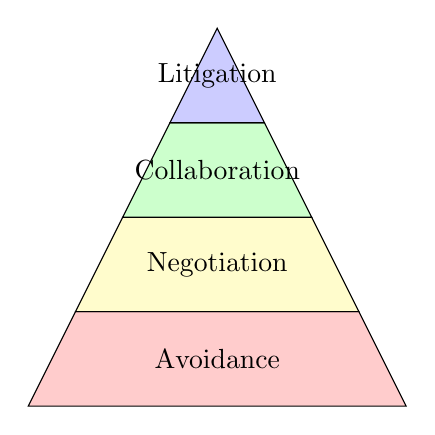
\begin{tikzpicture}[scale=1.2]
            % Draw pyramid levels
            \draw[fill=red!20] (-2,0) -- (2,0) -- (1.5,1) -- (-1.5,1) -- cycle;
            \draw[fill=yellow!20] (-1.5,1) -- (1.5,1) -- (1,2) -- (-1,2) -- cycle;
            \draw[fill=green!20] (-1,2) -- (1,2) -- (0.5,3) -- (-0.5,3) -- cycle;
            \draw[fill=blue!20] (-0.5,3) -- (0.5,3) -- (0,4) -- (-0,4) -- cycle;
            
            % Add labels
            \node at (0,0.5) {Avoidance};
            \node at (0,1.5) {Negotiation};
            \node at (0,2.5) {Collaboration};
            \node at (0,3.5) {Litigation};
        \end{tikzpicture}
    \end{center}
    
    \begin{block}{Key Insight}
        Strategies should match the conflict's scale and importance
    \end{block}
    \note{
        \begin{itemize}
            \item The conflict resolution pyramid illustrates different strategies for managing policy conflicts, ranging from avoidance at the base to litigation at the top.
            \item The key insight is that strategies should match the scale and importance of the conflict. For minor disputes, avoidance or negotiation may be sufficient, while more significant conflicts may require collaboration or litigation.
            \item By understanding the conflict resolution pyramid, policymakers can choose appropriate strategies to address policy disputes effectively and achieve positive outcomes.
            \item The conflict resolution pyramid offers a framework for selecting appropriate strategies based on the scale and importance of the conflict. It helps policymakers navigate disputes and reach successful resolutions.
            \item The Conflict Resolution Pyramid shows how strategies vary in intensity and resource needs. Choosing the right approach depends on the conflict's nature and stakes.
        \end{itemize}
    }
\end{frame}

\begin{frame}{Summary of Key Insights}
    \begin{columns}[T]
        \begin{column}{0.5\textwidth}
            \textbf{Conflict Sources:}
            \begin{itemize}
                \item Stakeholder interests
                \item Ideology
                \item Resources
                \item Regulations
            \end{itemize}
        \end{column}
        \begin{column}{0.5\textwidth}
            \textbf{Management Strategies:}
            \begin{itemize}
                \item Negotiation
                \item Mediation
                \item Collaboration
                \item Litigation
            \end{itemize}
        \end{column}
    \end{columns}
    
    \begin{alertblock}{Opportunities}
        Innovation \faIcon{lightbulb} \quad
        Engagement \faIcon{users} \quad
        Stronger Institutions \faIcon{building}
    \end{alertblock}
    \note{
        \begin{itemize}
            \item Policy conflicts arise from differing stakeholder interests, ideological divides, resource constraints, and regulatory challenges. Understanding these sources is key to effective conflict management.
            \item Policymakers can use negotiation, mediation, collaboration, and litigation to address policy conflicts and reach positive outcomes. Each strategy offers unique benefits and challenges.
            \item Conflict can be an opportunity for innovation, engagement, and building stronger institutions. By managing conflicts effectively, policymakers can turn challenges into opportunities for positive change.
            \item Policy conflicts are complex and multifaceted, requiring careful analysis and strategic management. By understanding the sources of conflict and using appropriate strategies, policymakers can navigate disputes effectively and achieve positive outcomes.
        \end{itemize}
    }
\end{frame}

\begin{frame}{Tips for Managing Policy Conflicts}
    \begin{columns}[T]
        \begin{column}{0.5\textwidth}
            \textbf{Skills to Develop:}
            \begin{itemize}
                \item Negotiation \faIcon{handshake}
                \item Communication \faIcon{comments}
            \end{itemize}
        \end{column}
        \begin{column}{0.5\textwidth}
            \textbf{Strategies to Adopt:}
            \begin{itemize}
                \item Flexibility \faIcon{sync}
                \item Evidence-based \faIcon{chart-line}
            \end{itemize}
        \end{column}
    \end{columns}
    
    \begin{exampleblock}{Key Focus}
        Building trust and maintaining open communication
    \end{exampleblock}
    \note{
        \begin{itemize}
            \item To manage policy conflicts effectively, develop negotiation and communication skills. These abilities are essential for building trust and reaching agreements among stakeholders.
            \item Adopt strategies like flexibility and evidence-based decision-making to address conflicts and adapt to changing circumstances. These approaches can help you navigate disputes and achieve positive outcomes.
            \item Focus on building trust and maintaining open communication with stakeholders. These practices are key to managing policy conflicts and fostering collaboration among diverse groups.
            \item Effective conflict management requires strong negotiation and communication skills, as well as flexibility and evidence-based decision-making. By focusing on building trust and open communication, policymakers can navigate conflicts successfully and achieve positive outcomes.
        \end{itemize}
    }
\end{frame}

\begin{frame}{Final Reflection Questions}

    \begin{enumerate}
    \item Drawing on specific examples from environmental or healthcare policy, analyze how competing stakeholder interests shape policy outcomes. How do different conflict management strategies affect the balance between economic and social goals?
    
    \bigskip
    
    \item Compare and contrast the effectiveness of litigation versus collaborative approaches in resolving policy conflicts, using historical examples from civil rights or environmental policy. What factors determine which approach is more likely to succeed?
    
    \bigskip 
    
    \item Evaluate how resource limitations and ideological differences intersect to create policy conflicts in social welfare programs. How do these constraints affect the choice between comprehensive versus incremental policy solutions?
    
    \bigskip
    
    \item Analyze the role of federalism in creating and resolving policy conflicts. Using examples from drug policy or environmental regulation, discuss how intergovernmental tensions influence policy implementation and outcomes.
    \end{enumerate}
    
    \note{
     Questions test understanding of:
     - Core policy conflict concepts
     - Real-world applications
     - Critical analysis of management strategies
     - Institutional factors in policy conflicts
     - Trade-offs between approaches
    }
    
    \end{frame}

\begin{frame}
    \begin{center}
        \Huge See You Next Time!
    \end{center}
\end{frame}

\begin{frame}{Role-Play: Negotiating a Policy Conflict}
    \begin{block}{Scenario}
        Negotiating climate change policy among stakeholders
    \end{block}
    
    \begin{columns}[T]
        \begin{column}{0.33\textwidth}
            \centering
            \textbf{Industry}\\
            \faIcon[3x]{industry}\\
            Economic Growth
        \end{column}
        \begin{column}{0.33\textwidth}
            \centering
            \textbf{Activist}\\
            \faIcon[3x]{leaf}\\
            Environment
        \end{column}
        \begin{column}{0.33\textwidth}
            \centering
            \textbf{Government}\\
            \faIcon[3x]{balance-scale}\\
            Balance
        \end{column}
    \end{columns}
    
    \begin{alertblock}{Task}
        Develop a policy proposal acceptable to all parties
    \end{alertblock}
    \note{
        \begin{itemize}
            \item In this role-play activity, students will negotiate a climate change policy among stakeholders with competing interests.
            \item Each group represents a different stakeholder—industry, activists, and government—each with distinct priorities and goals.
            \item The task is to develop a policy proposal that balances economic growth, environmental protection, and regulatory concerns to reach a consensus among all parties.
            \item The negotiation role-play will help students understand the complexities of policy conflicts and the challenges of reaching agreement among diverse stakeholders.
        \end{itemize}
    }
\end{frame}

\begin{frame}{Post-Activity Reflection}
    \begin{exampleblock}{Discussion Questions}
        \begin{enumerate}
            \item What strategies worked best in your role?
            \item What challenges did you face in reaching agreement?
            \item How do power imbalances affect real-world negotiations?
        \end{enumerate}
    \end{exampleblock}
    
    \begin{center}
        \faIcon[3x]{comments}
    \end{center}
    \note{
        \begin{itemize}
            \item After the negotiation activity, students will reflect on their experiences and discuss the challenges and strategies that emerged during the role-play.
            \item The discussion questions will prompt students to consider the effectiveness of different negotiation strategies, the challenges of reaching agreement, and the impact of power imbalances on real-world negotiations.
            \item By reflecting on their negotiation experiences, students can gain insights into the complexities of policy conflicts and the strategies needed to manage them effectively.
            \item After the role-play, reflect on the challenges and successes you experienced. Think about how these dynamics mirror real-world policy negotiations.
        \end{itemize}
    }
\end{frame}

\end{document}